\begin{dbltab}
   \begin{center}
\footnotesize\begin{tabular}{ | l || c | c | c | c | c | c | c | c | c | c |}
\hline
\multirow{2}{*}{\textbf{Program}} & \multicolumn{5}{c |}{\textbf{Queue
   Instructions}} & \multicolumn{5}{c |}{\textbf{Facts Derived}} \\ \cline{2-11}
& 1 & 2 & 4 & 8 & 16 & 1 & 2 & 4 & 8 & 16\\ \hline
\hline
SSSP - Regular & 199.1K & 203.1K & 202.7K & 203.8K & 206.4K & 3.3M & 3.0M & 3.4M & 3.5M & 3.3M \\
SSSP - Coordinated & 959.0K & 924.3K & 891.0K & 966.3K & 1.0M & 2.0M & 2.3M & 2.3M & 2.2M & 2.3M \\
SSSP - Buffered & 1.0M & 1.0M & 1.1M & 1.0M & 1.1M & 2.0M & 2.1M & 2.3M & 2.3M & 2.4M \\
\hline
HT - Regular & 25.6M & 33.3M & 34.8M & 36.1M & 34.8M & 235.7M & 298.3M & 312.1M & 317.5M & 310.3M \\
HT - Coordinated & 51.6M & 55.2M & 85.9M & 79.9M & 75.6M & 129.2M & 183.4M & 254.1M & 242.0M & 252.4M \\
HT - Local-Only & 51.6M & 54.9M & 81.0M & 76.7M & 67.3M & 129.2M & 180.8M & 221.5M & 217.6M & 207.4M \\
\hline
LBP - Regular & 15.7M & 17.8M & 16.0M & 11.3M & 8.5M & 160.2M & 171.0M & 149.9M & 107.5M & 85.1M \\
SBP - Coordinated & 97.2M & 97.4M & 90.0M & 84.3M & 79.2M & 76.8M & 80.7M & 79.2M & 79.0M & 79.3M \\
\hline \hline
MiniMax - Regular & 16.4M & 18.3M & 20.5M & 19.4M & 20.9M & 76.4M & 76.4M & 76.4M & 76.4M & 76.4M \\
MiniMax - Coordinated & 52.0M & 52.0M & 52.0M & 52.0M & 52.0M & 76.4M & 76.4M & 76.4M & 76.4M & 76.4M \\
\hline
N Queens - Regular & 8.4K & 14.4K & 17.7K & 16.6K & 19.3K & 167.1M & 167.1M & 167.1M & 167.1M & 167.1M \\
N Queens - Coordinated & 57.1M & 24.7M & 1.1M & 141.1K & 41.6K & 167.1M & 167.1M & 167.1M & 167.1M & 167.1M \\
N Queens - Static & 57.1M & 47.2M & 3.4M & 1.5M & 209.2K & 167.1M & 167.1M & 167.1M & 167.1M & 167.1M \\
\hline
\end{tabular}
\vspace*{.5ex}
\end{center}
\scap{queue_instructions}{Total number of queue \scare{instructions} and facts derived per program. An
   operation to a regular queue counts as 1 instruction, while an operation to
   a priority queue costs the number of
   \emph{percolate-up}/\emph{percolate-down} steps performed.}
\end{dbltab}

Coordination introduces overhead in two major ways.  First, in
manipulating the priority queues which require operations on a min
heap.  Second, in potentially requiring more lock operations as we
move nodes between queues and within the priority queue.  As we show
next, this overhead is minimal and is compensated by the resulting improved schedules
and memory locality that more than make up for the overhead.

As can be seen in Table~\ref{queue_instructions} all the coordinated
versions of the programs require significantly more queue operations.
The data for this table comes from recording the number of \emph{queue instructions} and the number of facts derived.
Queue instructions represent the
number of normal queue operations executed (each costs 1) plus the
number of \emph{percolate-up}/\emph{percolate-down} operations
executed for each manipulation of the priority queue.  As expected,
programs which rely on prioritizing the order of execution to obtain
better asymptotic complexity (e.g., SSSP) improve in overall running
time at the cost of more queue operations.  In all cases, coordination
adds a significant number of total queue operations, but the resulting
overhead is more than compensated for by an improved schedule and reduction
in number of facts produced. For MiniMax and N Queens, the number of facts derived
is the same for all configurations, as expected. The performance seen for those programs
arise from reduced memory usage and improved memory locality.

An interesting artifact of effectively parallelizing the code is that
the priority queue on each thread is smaller, so the total number of
priority queue operations is significantly reduced as the depth of the
min heap on each thread is reduced.  This is particularly evident for
the N Queens program.

\begin{topfig}
   \begin{center}
      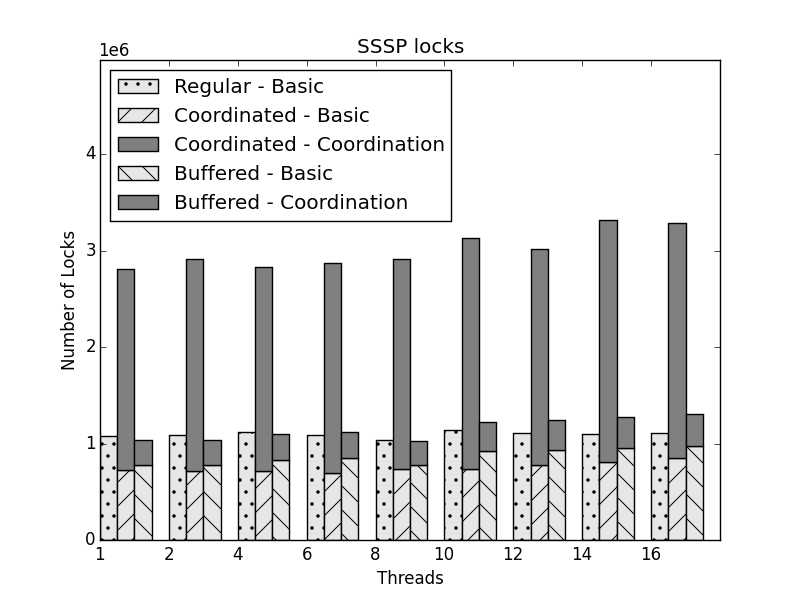
\includegraphics[width=6.5cm]{results/locks/sssp-locks.png}
   \end{center}
  \scap{locks:SSSP}{Locking statistics for SSSP.
     \texttt{Coordinated} refers to the program in
     Fig.~\ref{results:sssp_uspowergrid}, while \texttt{Buffered} is a more
     optimized version of the same program where coordination operations are
     buffered before application.}
\end{topfig}

\begin{topfig}
   \begin{center}
      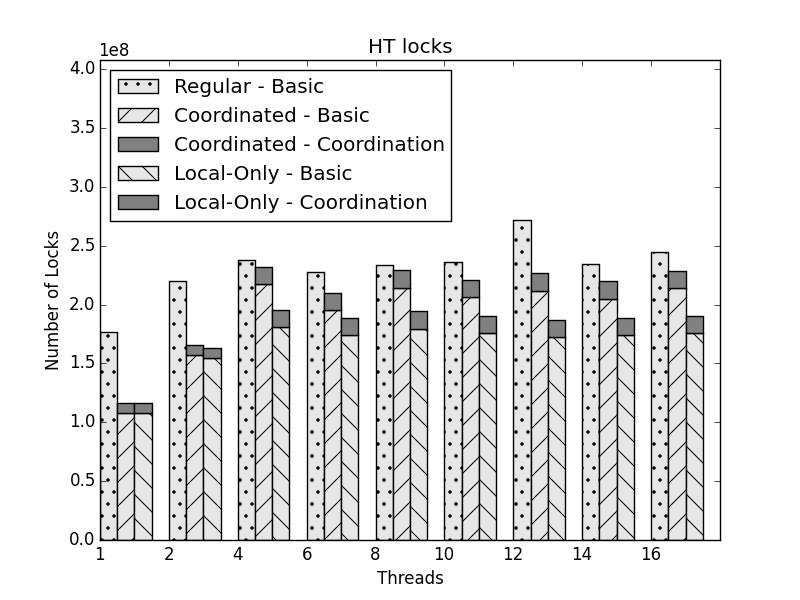
\includegraphics[width=6.5cm]{results/locks/ht-locks.png}
   \end{center}
  \scap{locks:HT}{Locking statistics for HT. Coordination reduces
     the overall number of locks used, while further optimization for locality
     reduces the locks even further.}
\end{topfig}

We next investigate the effect of coordination on the synchronization
overhead that comes from the use of more locks.  We measured the
\emph{basic locks}, the number of locks acquired
in the original LM virtual machine and \emph{coordination locks}, the
number of locks acquired to perform coordination operations.  We also
measured how often \texttt{lock()} operations that fail to acquired
the lock on the first attempt.  Lock failures happen so infrequently
(less than 1\% of the time) that they cannot be seen on the figures.

Fig.~\ref{results:sssp_uspowergrid} shows the number of locks acquired
for the SSSP program.  The first bar in each group shows the number of
locks acquired for the regular version of the program.  The
second bar shows the basic and coordination locks acquired for the coordinated
version of SSSP when every newly derived fact and priority operation is carried out
immediately.  This leads to a significant increase in total locks
acquired often because the priority of a node is change many times
before it is operated on.  The third bar shows the effect of buffering
priority operations before applying them.  This significantly reduces
the lock overhead, but as can be seen in
Table~\ref{queue_instructions}, increases the number of queue operations
slightly.  This slight increase comes from the fact that buffering
delays the change in priorities and some longer paths can sometimes be
investigated unnecessarily.

Fig.~\ref{locks:HT} shows the locking behavior of the heat transfer
program.  The behavior is representative of the other programs. In general, there
is a drop in the total number of locks acquired and coordination locks
represent a small fraction of the total number of locks acquired.  The \textbf{Local-Only}
version further reduces locking by keeping more derivations local
to a thread.

Overall, the additional overhead introduced by supporting coordination
is more than offset by improved schedules and increased locality.
While there are more locks to manage the total cost of lock operations,
the numbers do not change significantly (and is often reduced) when coordination
is added.  And, although the priority coordination significantly
increases the cost of queueing it is offset by reducing the number of
total facts derived.


\iffalse

  The
SSSP program is The first program we measured was SSSP, represented in
Fig.~\ref{results:sssp_uspowergrid}. In addition to the Regular and
Coordinated versions, we have the Buffered version where we optimized
the virtual machine to buffer coordination actions before applying
them. The idea is to avoid applying multiple \texttt{set-priority}
operations to the same node during a single node execution. We thus
gather the higher priority values and then perform coordination after
the node has executed.  Although the number of locks is significantly
reduced, we did not see a similar performance improvement, since the
Buffered version is only 5\% faster than the Coordinated version.


In Fig.~\ref{locks:HT} we show the lock statistics for HT. We measured the
regular version, the coordinated version and the local-only version as in
Fig.~\ref{results:ht}. There is a slight reduction in number of locks with
coordination and then a further reduction in the local-only version because less
facts are exchanged between threads.

Finally, in Fig.~\ref{locks:LBP} we present lock statistics for LBP and SBP. LBP
is represented as the Regular bar, while SBP is represented as the Coordinated
bar. We notice that LBP has quite a lot of locking for 1 thread since LBP
is an asynchronous algorithm and tends to be a slow sequential algorithm,
requiring more derivations when using 1 thread. The numbers go down as more
threads are used. For SBP, there is a consistent amount of locking without
little variations between the number of threads used. This is because threads
interact very little with each other and the amount of work to do is the same
for all threads.

\begin{topfig}
   \begin{center}
      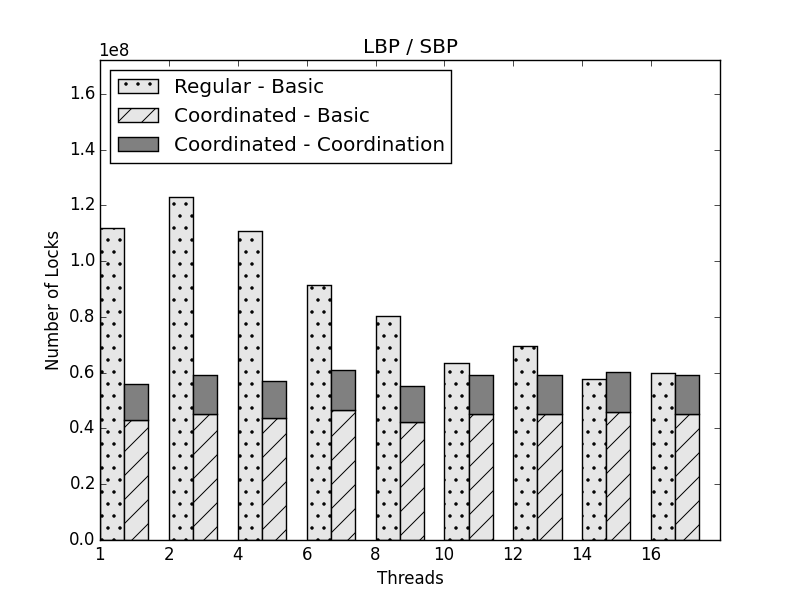
\includegraphics[width=6.5cm]{results/locks/bp.png}
   \end{center}
  \scap{locks:LBP}{Locking statistics for LBP and SBP. Locking is constant for
     SBP because threads do not interact with each other.}
\end{topfig}

\paragraph{Queue Instructions}

Table~\ref{queue_instructions} presents the total queue instructions for several
programs. All the coordinated programs require far more queue instructions than
the regular version. For instance, the coordinated SSSP program requires 4 to 5
times more instructions to perform queue operations. Interestingly, the buffered
version requires even more instructions although it performs less overall
coordination. It is likely that this is due to increased fact computation and
subsequent queue manipulation because coordination operations are buffered.
We argue that the 5\% performance improvement in the
buffered version is due mostly to reduced locking.

For the HT program, the coordinated version requires twice more queue
instructions than the regular version. As expected, the local-only version
requires less queue operations because the number of derived facts is reduced.
The MiniMax program also sees twice as many queue instructions using
coordination. This does not happen with the N Queens program, where the number
of queue instructions is far greater when using coordination, especially when
using a small number of threads. We argue that this happens because higher
priority nodes at the bottom are often added to the priority queue, resulting in
many \emph{percolate-up} operations.

These experiments indicate that handling coordination has a small cost in terms
of synchronization but some cost in terms of queue operations with
up to 5 times more queue instructions when using priority queues.
Since coordination reduces the number of facts derived due to better scheduling
decisions, the costs of manipulating priority queues become irrelevant.
\fi
